\subsection{Pixel-Space Video Forecasting}\label{sec:video-main}
We also evaluate KTH human-action videos and CLEVRER object-motion videos, using FVD as in \citet{chen2024forecasting}. This pilot predicts $64\times64$ pixels directly and conditions on the last $N$ consecutive frames. KTH uses grayscale frames with $N=10$ observations and $30$ forecasts; CLEVRER uses RGB, $N=2$, and $14$ forecasts at stride five. All four model families are trained separately on each dataset. The stochastic-interpolant and flow-matching teachers start from scratch; each map is initialized and trained from its own newly trained teacher. The selected models use the same 128 frozen test clips and four sampled completions per clip. FVD embeds the observed prefix together with the future, using a fixed pretrained I3D detector. Our pooled comparison has 128 real and 512 generated clips, versus 256 and 25,600 in the original study; it is a smaller pixel-space pilot, not a numerical reproduction of the latent-space benchmark. Appendix~\ref{app:video-case} gives the training and metric protocol.

\IfFileExists{generated/video_main_results.tex}{%

\begin{table*}[t]\centering\small
\begin{tabular}{lrrrrr}
\toprule
Model & NFE/frame & KTH pooled & KTH member & CLEVRER pooled & CLEVRER member \\
\midrule
SI & 16 & 1781.7 & 1812.6 $\pm$ 16.3 & 436.1 & 485.3 $\pm$ 16.2 \\
SI & 64 & 773.5 & 823.0 $\pm$ 20.7 & 222.3 & 268.9 $\pm$ 10.7 \\
FM & 16 & 726.8 & 766.9 $\pm$ 17.2 & 323.0 & 361.8 $\pm$ 19.1 \\
FM & 64 & 783.1 & 831.5 $\pm$ 21.7 & 330.0 & 372.1 $\pm$ 19.8 \\
It\^o map & 1 & 1271.3 & 1302.2 $\pm$ 18.8 & 1080.0 & 1117.4 $\pm$ 18.9 \\
It\^o map & 8 & 888.2 & 926.5 $\pm$ 21.1 & 317.3 & 360.5 $\pm$ 6.0 \\
Flow map & 1 & 857.2 & 895.1 $\pm$ 18.1 & 402.2 & 442.7 $\pm$ 5.4 \\
Flow map & 8 & 706.6 & 748.0 $\pm$ 19.0 & 320.4 & 359.9 $\pm$ 15.3 \\
Persistence & 0 & 816.1 & 815.8 $\pm$ 0.0 & 1072.2 & 1071.5 $\pm$ 0.0 \\
\bottomrule
\end{tabular}

\caption{Pixel-video FVD (lower is better). Pooled FVD compares 128 real and 512 generated clips. Member FVD reports mean $\pm$ completion SD of four separate 128-versus-128 comparisons, not confidence intervals. Cases are shared; each model uses one checkpoint at all its budgets. NFE is per generated frame and member; persistence uses none. Other metrics are in Appendix~\ref{app:video-results}.}\label{tab:video-main-fvd}
\end{table*}
\begin{figure*}[t]\centering
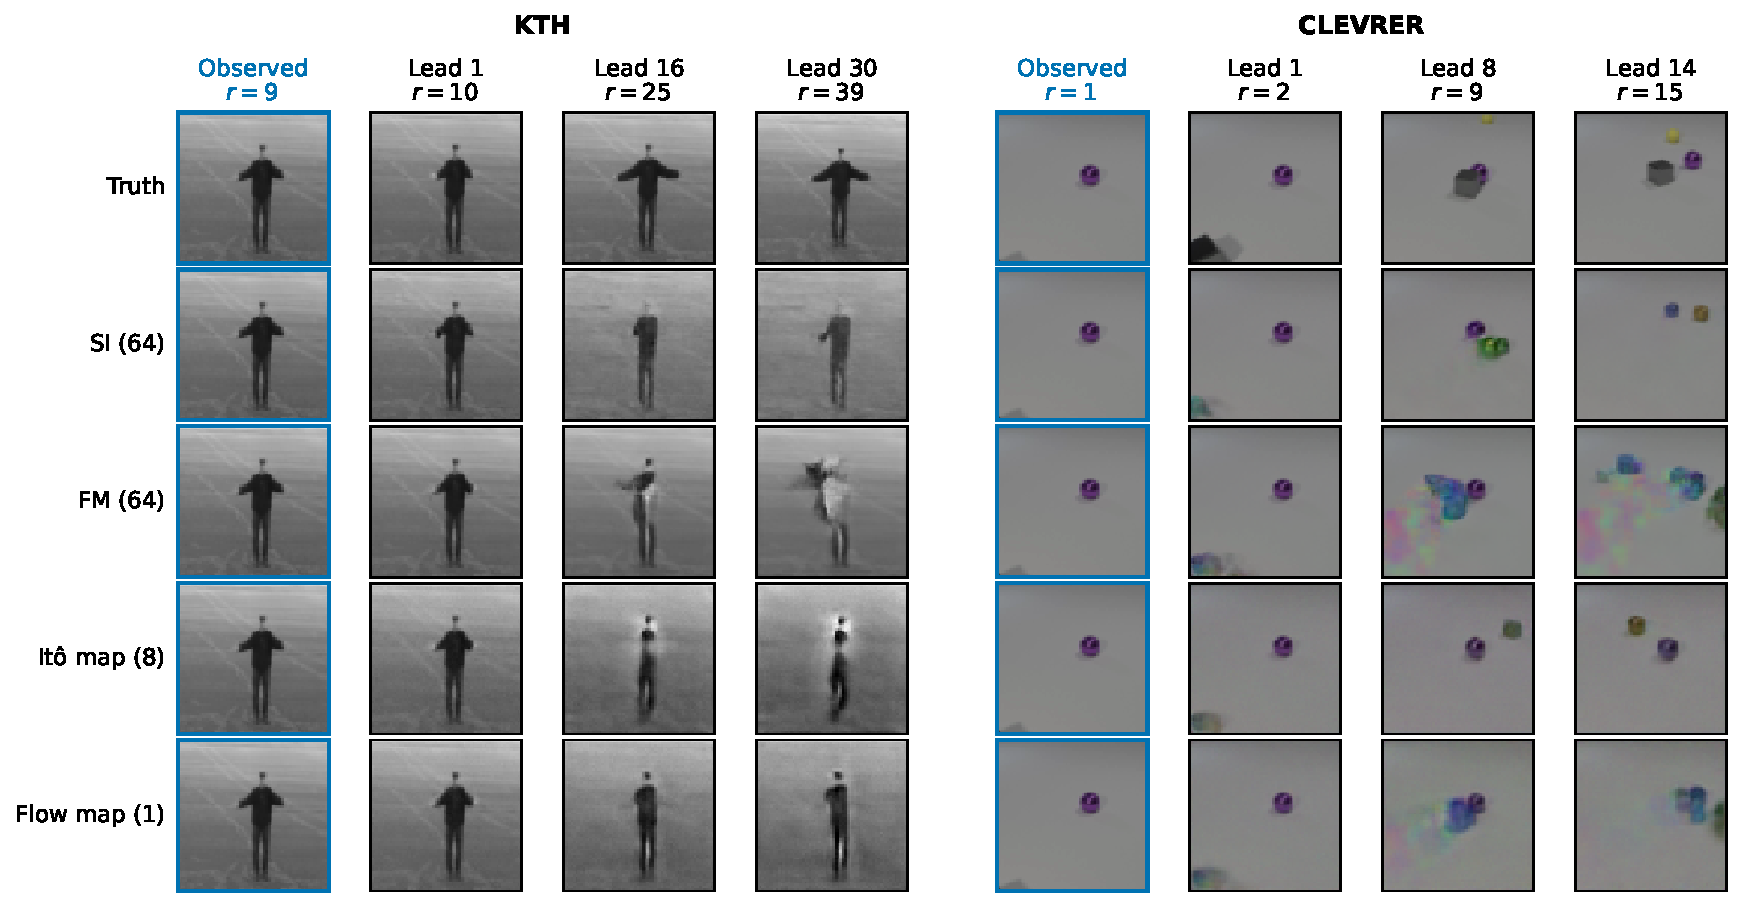
\includegraphics[width=\textwidth]{figures/video_results/main_forecast_sequences.pdf}
\caption{Matched observed and predicted frame sequences for both datasets. Rows show truth and one sampled completion from each model, never an ensemble average. The blue-bordered column repeats the last observed frame; remaining columns are forecasts. $r$ is the zero-based retained-frame index within the clip: KTH retains every frame; CLEVRER raw-frame index is $5r$. Cases are the first frozen selections, member zero, at prespecified budgets (parentheses). Display clipping does not alter feedback. The other observed history frames condition each model but are omitted for space.}\label{fig:video-main-sequences}
\end{figure*}
%
}{%
All eight dataset/model combinations have completed training and were frozen before testing. The matched all-model evaluation is still running. Its FVD comparison and fixed truth-versus-prediction frame sequences for both datasets will be included only after both artifact audits pass; no video-quality conclusion is drawn from incomplete results.
}
